% \section*{Potential Risks}

% This work improves the efficiency of long-context LLM inference, so its main potential risk is that lower latency and serving cost may also facilitate undesirable uses of existing language models, such as large-scale generation of misleading, abusive, or otherwise harmful content. This risk is not specific to our compressed-memory design, but applies broadly to inference acceleration techniques. Our method does not introduce a new user-facing model, collect new human-subject data, or modify the target model distribution: the target verifier keeps its standard full KV cache and applies the usual speculative decoding accept/reject rule, so the output distribution remains identical to vanilla target-model decoding. Therefore, the proposed compressed draft-side memory primarily affects inference efficiency rather than the semantic behavior or safety properties of the target model. In deployment, it should be used together with the same content moderation, access control, and monitoring mechanisms required for the underlying model.


\section{Scientific Artifacts}
\label{sec:scientific-artifacts}

This work uses existing scientific artifacts, including publicly available research models and datasets, solely for research and evaluation purposes. We cite the original creators of the models, datasets, baselines, and software frameworks used in our experiments in the corresponding experimental setup and baseline sections, as well as in the references. We use these artifacts consistently with their stated intended uses and access conditions, and we follow the licenses or terms specified by their original providers.

We do not collect new human-subject data, annotate private data, or redistribute raw datasets. The datasets used in our experiments are standard public research benchmarks. To the best of our knowledge, based on their original documentation, these datasets are not intended to contain personally identifying information. Since our work focuses on efficiency evaluation rather than dataset construction, we rely on documentation from the original artifact creators for details such as data source, domain, language coverage, and usage restrictions. We also document the models, datasets, evaluation settings, and implementation details used in our experiments.

\section{Potential Risks}

MASW accelerates inference but does not add new content-generation capabilities, and it inherits the safety, bias, and privacy risks of its underlying models and training data.
Greater inference efficiency may nevertheless enable harmful uses of existing models at a larger scale.
The lossless guarantee also relies on verifying every draft proposal with the target model; deployments that weaken or bypass this verification may change model outputs.
Practitioners should therefore retain full target verification and apply the same access controls, monitoring, and content safeguards required for the underlying model.

\newpage
\section{Memory Prefill}
\label{sec:memory-prefill}

\begin{figure}[h]
    \centering
    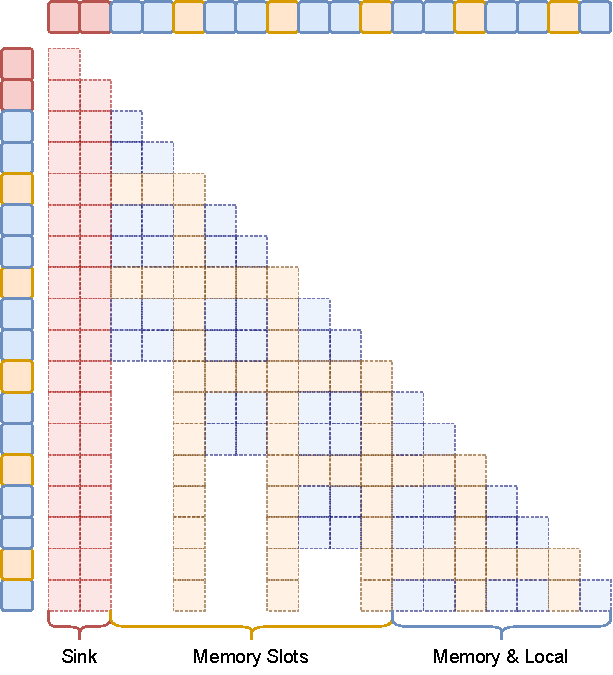
\includegraphics[width=0.85\linewidth]{fig/EMNLP-Mask.drawio.pdf}
    \caption{Memory prefill attention mask.}
    \label{fig:memory_prefill}
\end{figure}

During draft-side prefill, the attention mask enforces the same memory-write policy used during decoding.
Sink tokens remain globally visible to stabilize attention, and each memory-slot token can attend to previously materialized slots together with the raw tokens in its assigned local unit and neighboring boundary tokens.
Ordinary raw tokens, in contrast, are restricted to the compact memory view: sink tokens, available memory slots, and the bounded local window.
This asymmetric visibility lets the prefill pass build the initial compressed memory $\mathcal{M}_t$ while avoiding a full raw-token KV cache for the draft model.
Figure~\ref{fig:memory_prefill} illustrates this mask structure.

\section{Detailed Experimental Setting}
\label{sec:detailed-experimental-setting}

% \paragraph{Scope of baseline comparisons.}
% All reported baseline results are reproduced within the same Hugging Face Transformers framework.
% TokenSwift~\citep{wu2025tokenswift} combines sparse Medusa heads with several end-to-end system optimizations.
% We do not compare its published end-to-end speedups with our component-level baselines because such a comparison would conflate draft-memory quality with orthogonal system optimizations.

% \paragraph{Table-specific configuration.}
% The ``8B draft, with memory'' row in Table~\ref{tab:prefill_latency} uses nominal 8$\times$ compression with $W=S=128$.

% \paragraph{Training configuration.}
% We use AdamW with a peak learning rate of $10^{-5}$.
% The rate warms up linearly from zero over 256 steps and then follows a cosine schedule to 50\% of its peak.
% For SFT, we retain the optimizer and learning-rate scale but reduce warm-up to 128 steps.
% The slot interval and local-window size remain fixed throughout training.

\paragraph{Component-level baselines.}
We reproduce SWA and SnapKV within the same Hugging Face Transformers framework~\citep{wolf-etal-2020-transformers}.
For both baselines, the draft and target use the same model backbone and weights.
The draft generates tokens autoregressively using SWA or SnapKV for draft-side KV reduction, whereas verification uses the full target KV cache.
SWA uses a sliding-window size of 1,024 tokens.
SnapKV retains 4,096 KV entries and otherwise follows its official default configuration.
For EAGLE and EAGLE-3, we use chain-based proposal generation with the released checkpoints and the remaining official inference settings.
All speculative methods in Table~\ref{tab:main_results_long_input} propose five draft tokens per iteration; the separate motivation experiment in Figure~\ref{fig:motivation_eagle_throughput_vs_context_length} uses a 10-token proposal horizon.

\paragraph{Decoding and timing.}
The reported 8K, 16K, 24K, and 32K lengths refer to the input prefix before generation and exclude output tokens.
We filter examples from GovReport, QMSum, and MultiNews whose tokenized inputs match the evaluated prefix length.
Each run generates at most 1,024 output tokens and stops early when the model emits an end-of-sequence token.
\textit{Tok./Iter} denotes the mean number of tokens emitted per speculative iteration.
Decoding throughput (\textit{tok/s}) is the number of generated output tokens divided by decoding wall-clock time; draft and target prefill are excluded.
\textit{Speedup} denotes decoding speedup over the corresponding AutoRegressive baseline under the same prefix length and timing scope.

\begin{comment}
\section{Results on Qwen2.5 Models}

\begin{table*}[t!]
    \centering
    \resizebox{\textwidth}{!}{%
    \begin{tabular}{@{}l|l|ccc|ccc|ccc|ccc@{}}
        \toprule
        & & \multicolumn{3}{c|}{8K} & \multicolumn{3}{c|}{16K} & \multicolumn{3}{c|}{24K} & \multicolumn{3}{c}{32K} \\
        & & Tok./Iter & tok/s & Speedup & Tok./Iter & tok/s & Speedup & Tok./Iter & tok/s & Speedup & Tok./Iter & tok/s & Speedup \\
        \midrule
        & SWA                &  &  & 0.87$\times$ &  &  & 0.52$\times$ &  &  & 0.59$\times$ &  &  & 0.55$\times$ \\
        & SnapKV             &  &  & 0.91$\times$ &  &  & 0.99$\times$ &  &  & 1.18$\times$ &  &  & 1.31$\times$ \\
        & SD Q7B             &  &  & 2.11$\times$ &  &  & 2.13$\times$ &  &  & 1.95$\times$ &  &  & 2.02$\times$ \\
        \rowcolor[gray]{0.9}\cellcolor{white}
        \multirow{-4}{*}{\rotatebox{90}{Q2.5-72B}}
        & Ours 8$\times$ Q7B &  &  & 2.95$\times$ &  &  & 2.57$\times$ &  &  & 2.48$\times$ &  &  & 2.36$\times$ \\
        \bottomrule
    \end{tabular}%
    }
    \caption{Preliminary long-input speculative decoding results on the Qwen2.5 model family. The target is Qwen2.5-72B, and SD and MASW use Qwen2.5-7B as the draft model. \textit{Tok./Iter} denotes the mean number of tokens emitted per speculative iteration; \textit{tok/s} denotes decoding throughput, and \textit{Speedup} is relative to the AutoRegressive baseline.}
    \label{tab:qwen25_results_long_input}
\end{table*}
\end{comment}

\FloatBarrier


% \newpage
% \section{Experimental Details}

% \subsection{Setup and Hyper-parameters}

% \subsection{Draft Quality}

% % * Draft Quality ($\tau$)

% \subsection{Draft Speed}

% % * Draft Speed (Tokens/s)

% \clearpage
\section{Notations}

\begin{table*}[h]
    \centering
    \resizebox{\textwidth}{!}{%
    \begin{tabular}{@{}lll@{}}
        \toprule
        Part & Notation & Explanation \\
        \midrule
        Speculative decoding & $\mathsf{M}_d$, $\mathsf{M}_t$ & draft and target models \\
                              & $L_{\text{draft}}$ & number of draft tokens proposed per iteration; fixed to 5 \\
                              & $L_{\mathrm{acc}}$ & mean number of accepted draft tokens per iteration \\
                              & $L_{\mathrm{emit}}$ & mean emitted tokens per nonterminal iteration; reported as Tok./Iter \\
                              & $t_d$, $t_t$ & single-token latency of the draft and target models \\
        \midrule
        Draft memory & $\mathcal{D}_t$ & compact draft-side working memory at step $t$ \\
                     & $\mathcal{M}_{\mathrm{sink}}$ & exact KV for the first $S$ raw tokens \\
                     & $\mathcal{M}_{\mathrm{local},t}$ & exact raw-token KV in the local window \\
                     & $\mathcal{M}_{\mathrm{slot},t}$ & materialized KV entries for memory slots \\
                     & $\mathcal{S}=\{1,\ldots,S\}$ & sink-token positions \\
                     & $S$ & sink-token count \\
                     & $W$ & local-window width \\
                     & $r$ & slot interval; one slot per $r$ raw tokens \\
        \midrule
        Memory slots & $g_m$ & memory-slot token for unit $m$ \\
                     & $\tau_m=mr$ & compression boundary for slot $g_m$ \\
                     & $\mathcal{A}(g_m)$ & write scope of memory-slot token $g_m$ \\
                     & $\mathcal{G}_{<m}$, $U_m$, $\mathcal{N}_m$ & earlier slots, current unit, and neighboring tokens \\
        \midrule
        Transformer and KV & $d$ & hidden size \\
                           & $L$ & prefix length in the latency model \\
                           & $K_r^{(l)}$, $V_r^{(l)}$ & raw-token key and value at layer $l$ \\
                           & $K_g^{(l)}$, $V_g^{(l)}$ & memory-slot key and value at layer $l$ \\
                           & $W_{K,r}^{(l)}$, $W_{V,r}^{(l)}$ & frozen backbone KV projections for raw tokens \\
                           & $W_{K,g}^{(l)}$, $W_{V,g}^{(l)}$ & trainable mirrored KV projections for memory slots \\
                           & $W_{\ast,r}^{(l)}$, $W_{\ast,g}^{(l)}$ & shorthand for raw-token and memory-slot KV projections \\
        \bottomrule
    \end{tabular}
    }
    \caption{List of notation used in this paper.}
    \label{tab:notation}
\end{table*}
